%=============================================================================
% MicroAPI Guard - IEEE conference paper
%
% Build:
%   pdflatex microapi_guard
%   bibtex   microapi_guard
%   pdflatex microapi_guard
%   pdflatex microapi_guard
%
% Self-contained: every figure is drawn inline with TikZ/pgfplots, so no
% external image files are required.
%=============================================================================
\documentclass[conference]{IEEEtran}
\IEEEoverridecommandlockouts

\usepackage{cite}
\usepackage{amsmath,amssymb,amsfonts}
\usepackage{array}
\usepackage{booktabs}
\usepackage{tabularx}
\usepackage{graphicx}
\usepackage{textcomp}
\usepackage{xcolor}
\usepackage{float}
\usepackage{placeins}
\usepackage{stfloats}   % allows a double-column float at the bottom of its page
\usepackage{enumitem}
\usepackage[ruled,vlined,linesnumbered]{algorithm2e}
\usepackage{tikz}
\usetikzlibrary{shapes.geometric,shapes.multipart,arrows.meta,positioning,calc,fit,backgrounds}
\usepackage{pgfplots}
\pgfplotsset{compat=1.18}
\usepackage[hidelinks,bookmarks=false]{hyperref}

\newcolumntype{L}{>{\raggedright\arraybackslash}X}
\newcolumntype{P}[1]{>{\raggedright\arraybackslash}p{#1}}

% Palette used by every figure so the paper reads as one system.
\definecolor{srBlue}{HTML}{2A5D9F}
\definecolor{srTeal}{HTML}{2E8B8B}
\definecolor{srAmber}{HTML}{C8862B}
\definecolor{srGrey}{HTML}{6B7280}
\definecolor{srLight}{HTML}{EAF0F7}

\begin{document}

\title{MicroAPI Guard: A Four-Layer Stacking Ensemble \\
for Inline API Anomaly Detection \\ with \\
Session-Grouped Zero-Day Evaluation}

\author{%
\IEEEauthorblockN{Sunny Surendra Nirmal}
\IEEEauthorblockA{\textit{Dept. of Information Technology}\\
\textit{G H Raisoni College of Engineering \& Management}\\
Pune, India\\
sunny.nirmal.it@ghrcem.raisoni.net}
\and
\IEEEauthorblockN{Tausib Samir Patel}
\IEEEauthorblockA{\textit{Dept. of Information Technology}\\
\textit{G H Raisoni College of Engineering \& Management}\\
Pune, India\\
tausib.patel.it@ghrcem.raisoni.net}
\and
\IEEEauthorblockN{Yash Nandkumar Patil}
\IEEEauthorblockA{\textit{Dept. of Information Technology}\\
\textit{G H Raisoni College of Engineering \& Management}\\
Pune, India\\
yash.patil.it@ghrcem.raisoni.net}
\and
\IEEEauthorblockN{Priyanka Kumbhar}
\IEEEauthorblockA{\textit{Dept. of Information Technology}\\
\textit{G H Raisoni College of Engineering \& Management}\\
Pune, India\\
priyanka.kumbhar@raisoni.net}
}

\maketitle

\begin{abstract}
Application programming interfaces are the dominant attack surface of microservice
deployments, yet the available defences sit at opposite extremes. Signature firewalls are
deterministic and fast but blind to payloads nobody has written a rule for, while recent
learned detectors reach high accuracy using graph neural networks, language models or
distributed tracing pipelines that no request-path gateway can absorb. This paper presents
MicroAPI Guard, a backend-agnostic gateway composing four detection layers: 26 signature
rules with a Redis sliding-window rate limiter, a 300-tree Isolation Forest, a
3{,}314-parameter NumPy autoencoder, and a 107-iteration gradient-boosted meta-learner that
fuses the three anomaly scores into the single blocking decision. The deterministic layer
short-circuits, so cost tracks certainty: a rule verdict costs 47\,$\mu$s against 5.43\,ms
for the full path, a $116\times$ gap. We hold the evaluation to three constraints this
literature routinely relaxes---splits grouped by client session, a threshold fixed on
validation under a 1\% false-positive budget, and three attack families withheld from every
pool but test. Over ten session partitions the ensemble attains $F_1 = 0.957$
(95\% CI $[0.940,0.976]$) at a false-positive rate of $0.0069$, and recalls
$0.794\ [0.668,0.914]$ of attacks from families absent at training time; McNemar's test
rejects equality against every constituent detector ($\chi^2 \ge 152.3$, $p<10^{-34}$). Our
best partition reaches $F_1 = 0.991$ and zero-day recall $1.000$. We report the interval
instead, and argue the $0.426$--$1.000$ per-seed spread is the result worth stating. We also
show the fused decision boundary is non-monotonic in the base scores---explaining why a
linear meta-learner loses $0.275$ $F_1$, and flagging a transfer risk that recall-only
reporting hides.
\end{abstract}

\renewcommand{\IEEEkeywordsname}{Keywords}
\begin{IEEEkeywords}
API Security, Anomaly Detection, Microservices, Stacking Ensemble, Isolation Forest,
Autoencoder, Zero-Day Detection, API Gateway, Gradient Boosting.
\end{IEEEkeywords}

%=============================================================================
\section{Introduction}
Microservice architectures decompose an application into services that communicate almost
entirely over HTTP APIs. The security consequence is structural: the number of reachable
endpoints grows with the number of services, and each is a candidate entry point. Public
breach disclosures involving API misuse show that a single unmonitored route is sufficient
\cite{levi2026mrg}, and the OWASP API Security Top~10 \cite{owasp2023api} codifies the
resulting risk classes.

The difficulty is not writing a detector. It is deciding what a detector may cost. A gateway
sits on the request path, so every microsecond it spends is added to every response. Deployed
defences resolve this in one of two ways, and neither is satisfactory. Signature web
application firewalls are deterministic, fast and explainable, but recognise only attacks
somebody has already encoded as a rule---precisely the wrong property against novel or
obfuscated payloads \cite{levi2026mrg}. Learned detectors for microservice environments are
accurate but expensive: graph neural networks over service dependency graphs
\cite{liu2024lmgd}\cite{raeiszadeh2025artfl}, large language models over log streams
\cite{pedroso2025llm}, dynamic knowledge graphs \cite{moens2026kg}, or distributed tracing
pipelines \cite{liu2020traceanomaly}\cite{kohyarnejadfard2022nlp}. Each assumes infrastructure
absent from a gateway---a trace collector, a metrics pipeline, a GPU---and each measures
internal system health after the fact rather than the hostility of an inbound request before
it is forwarded.

\subsection{A Motivating Case}
\label{sec:case}
Consider two requests drawn from our corpus, both reaching the same endpoint template
\texttt{/api/products/\{id\}}, and both surviving Layer~1 with no rule hit. Their measured
detector scores are shown in Fig.~\ref{fig:case}.

\begin{figure}[H]
\centering
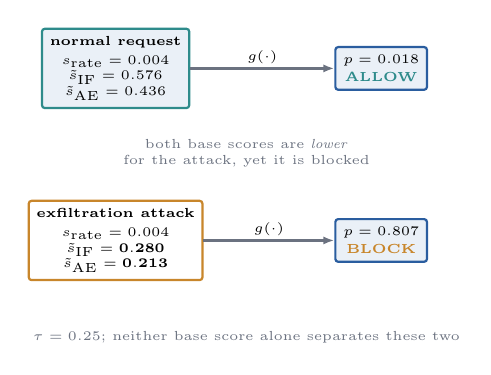
\begin{tikzpicture}[scale=0.95,transform shape,
  font=\tiny,
  box/.style={draw=srGrey,thick,fill=white,rounded corners=1pt,inner sep=3pt,align=center},
  benign/.style={box,draw=srTeal,fill=srLight},
  attack/.style={box,draw=srAmber,thick},
  meta/.style={box,draw=srBlue,fill=srLight,thick},
  ar/.style={-{Latex[length=1.4mm]},draw=srGrey,thick},
  el/.style={font=\tiny,inner sep=1.2pt,fill=white,align=center}]

\node[benign] (b) at (0,1.55)
  {\textbf{normal request}\\[1pt]$s_{\mathrm{rate}}=0.004$\\
   $\tilde{s}_{\mathrm{IF}}=0.576$\\$\tilde{s}_{\mathrm{AE}}=0.436$};
\node[attack] (a) at (0,-0.75)
  {\textbf{exfiltration attack}\\[1pt]$s_{\mathrm{rate}}=0.004$\\
   $\tilde{s}_{\mathrm{IF}}=\mathbf{0.280}$\\$\tilde{s}_{\mathrm{AE}}=\mathbf{0.213}$};

\node[meta] (mb) at (3.55,1.55) {$p=0.018$\\[1pt]\textcolor{srTeal}{\textbf{ALLOW}}};
\node[meta] (ma) at (3.55,-0.75) {$p=0.807$\\[1pt]\textcolor{srAmber}{\textbf{BLOCK}}};

\draw[ar] (b.east) -- node[el,above]{$g(\cdot)$} (mb.west);
\draw[ar] (a.east) -- node[el,above]{$g(\cdot)$} (ma.west);

\node[el,text=srGrey,align=center] at (1.75,0.42)
  {both base scores are \emph{lower}\\for the attack, yet it is blocked};
\node[el,text=srGrey] at (1.75,-2.05)
  {$\tau=0.25$; neither base score alone separates these two};
\end{tikzpicture}
\caption{Two real corpus requests on the same endpoint template, both passing Layer~1. The
attack scores \emph{lower} on both base detectors than the normal request, so no threshold on
either score---and no monotone combination of them---separates the pair. The gradient-boosted
meta-learner does.}
\label{fig:case}
\end{figure}

The normal request scores $0.576$ on the isolation forest and $0.436$ on the autoencoder. The
exfiltration attack scores \emph{lower on both}: $0.280$ and $0.213$. Any threshold on either
base score that blocks the attack also blocks the normal request, and so does any weighted sum
with positive coefficients. Yet the meta-learner assigns them $p=0.018$ and $p=0.807$
respectively, on either side of $\tau=0.25$.

This is why the choice of meta-learner is not cosmetic. Mapping the fused decision surface
(Section~\ref{sec:nonmono}) shows it is non-monotonic in the isolation-forest score over part
of its range, and a logistic-regression meta-learner---which cannot express such a region---
loses $0.275$ absolute $F_1$. It is also a warning: a boundary shaped like this fits the
training population tightly, and we report the resulting transfer risk rather than omitting it.

\subsection{Objectives}
This work is built around five objectives carried over from the project synopsis, restated to
match the system as finally implemented:

\begin{enumerate}[leftmargin=1.4em,itemsep=1pt,topsep=2pt]
  \item To design and implement a FastAPI reverse-proxy gateway that intercepts live HTTP
        traffic, extracts behavioural features through a Redis sliding window, and blocks
        malicious requests inline with HTTP~403 while forwarding legitimate traffic at
        minimal added latency.
  \item To train and deploy a heterogeneous stacking ensemble in which signature rules, an
        Isolation Forest and an autoencoder act as base detectors, with a learned
        meta-learner combining their anomaly scores into a decision more accurate than any
        standalone detector.
  \item To engineer a calibration phase that adapts the framework to unseen REST backends by
        observing a short window of normal traffic and updating statistical baselines and
        thresholds, without retraining from scratch.
  \item To evaluate the framework using Precision, Recall, $F_1$, ROC-AUC and PR-AUC averaged
        over multiple random seeds with 95\% confidence intervals, and to establish the
        significance of the ensemble's improvement over each base detector using McNemar's
        test.
  \item To make each layer's contribution inspectable, reporting the individual anomaly
        scores beside the final ensemble decision so that a verdict can be attributed to a
        layer rather than accepted as a single opaque number.
\end{enumerate}

\subsection{Summary of the Paper}
MicroAPI Guard is deployed in front of any HTTP backend by setting one environment variable;
nothing in the gateway knows the protected routes. Requests are normalised into a
34-dimensional feature vector describing request \emph{shape}, screened by a deterministic
layer that short-circuits on a hit, and---only if they survive---scored by two unsupervised
detectors whose outputs a gradient-boosted meta-learner fuses. We then report what recall-only
convention hides: per-layer cost, per-seed variance, and the shape of the fused boundary.

The remainder is organised as follows. Section~\ref{sec:lit} reviews eighteen studies
and states the gaps they leave. Section~\ref{sec:prob} makes the problem precise, and
Section~\ref{sec:arch} presents the system as a data-flow and a control-flow view.
Section~\ref{sec:method} gives the detection rules, the algorithms and the evaluation
protocol, Section~\ref{sec:results} reports the measurements, and Section~\ref{sec:concl}
concludes.

%=============================================================================
\section{Literature Review}
\label{sec:lit}
Table~\ref{tab:lit} summarises eighteen studies spanning microservice observability,
telemetry-based anomaly detection, gateway-level inspection and classical unsupervised
detectors. Each row records the objective, the method, the reported result and the gap left
open.

The works fall into three strands. The largest targets \emph{system health} from telemetry:
statistical decomposition of invocation chains \cite{jin2020rpca}, graph learning over logs
and metrics \cite{liu2024lmgd}, multimodal imputation for missing metrics
\cite{zhang2026admm}, deep Bayesian trace models \cite{liu2020traceanomaly}, NLP over traces
\cite{kohyarnejadfard2022nlp}, federated training \cite{raeiszadeh2025artfl}, language models
for root-cause analysis \cite{pedroso2025llm} and dynamic knowledge graphs \cite{moens2026kg}.
A smaller strand inspects traffic at the gateway \cite{sowmya2023api}\cite{huang2026gateway}
\cite{levi2026mrg}\cite{markande2026saas}. The third supplies the unsupervised detectors this
work reuses \cite{alshehari2023insider}\cite{sadaf2020autoif}\cite{mahmoud2025dsem} and the
zero-day protocol we adopt \cite{alam2025adaptive}.

\begin{table*}[!b]
\caption{Summary of the Reviewed Literature}
\label{tab:lit}
\centering
\scriptsize
\renewcommand{\arraystretch}{1.2}
\setlength{\tabcolsep}{4pt}
\begin{tabularx}{\textwidth}{@{}P{2.15cm}P{2.6cm}LP{2.9cm}P{2.75cm}@{}}
\toprule
\textbf{Reference} & \textbf{Objective} & \textbf{Method} & \textbf{Dataset / Key Result} &
\textbf{Research Gap} \\
\midrule
Sadaf \& Sultana, 2020 \cite{sadaf2020autoif} & Intrusion detection in fog &
Auto-IF: autoencoder $+$ isolation forest & NSL-KDD; 95.4\% accuracy &
Offline rows; no inline deployment \\
Jin et al., 2020 \cite{jin2020rpca} & Root cause in microservices &
RPCA on invocation chains, IF/OCSVM/LOF & AIOps 2020; score 0.8304 &
Metrics only; not request-level \\
Liu et al., 2020 \cite{liu2020traceanomaly} & Trace anomaly detection &
Service-level Bayesian model of normal traces & Production traces &
Needs full trace collection \\
Kohyarnejadfard et al., 2022 \cite{kohyarnejadfard2022nlp} & Performance anomalies &
NLP over distributed tracing spans & Real datasets; $F$-score 0.9759 &
Tracing infrastructure required \\
Al-Shehari et al., 2023 \cite{alshehari2023insider} & Insider threat under imbalance &
Anomaly-based isolation forest & CERT dataset &
Single detector; no ensemble \\
Sowmya et al., 2023 \cite{sowmya2023api} & API traffic anomalies &
ML on HTTP request features & Microservice testbed &
No zero-day protocol; no cost report \\
Liu et al., 2024 \cite{liu2024lmgd} & Multi-source detection &
LMGD: log--metric fusion on a service graph & $+2.63\%$ recall, $+1.05\%$ $F_1$ &
Off request path; GNN cost \\
Mahmoud et al., 2025 \cite{mahmoud2025dsem} & Reduce bias/variance in NIDS &
DSEM-NIDS deep stacking ensemble & 5G-NIDD, UNR-IDD, N-BaIoT, NSL-KDD &
Flow features; not API-aware \\
Alam et al., 2025 \cite{alam2025adaptive} & Zero-day detection &
Deep RL with stacked LSTM; classes withheld & Multiple NIDS benchmarks &
Heavy training; offline only \\
Raeiszadeh et al., 2025 \cite{raeiszadeh2025artfl} & Privacy-preserving detection &
ART-FL: async federated GNN with PU learning & Cloud microservice traces &
Requires edge training fleet \\
Pedroso et al., 2025 \cite{pedroso2025llm} & Root cause in cloud-native &
LLM with Bayesian networks, chaos injection & Kubernetes $+$ Istio testbed &
LLM inference cost prohibitive inline \\
Faseeha et al., 2025 \cite{faseeha2025observability} & Survey observability &
Frameworks, challenges, deployment paradigms & Systematic review &
Observability itself adds overhead \\
Barata et al., 2026 \cite{barata2026survey} & Survey detection and RCA &
117 studies, 2012--2025, taxonomy & Systematic review &
Scalability and real-time unresolved \\
Zhang et al., 2026 \cite{zhang2026admm} & Incomplete metrics &
ADmM: multi-scale AE imputation $+$ GNN & Three open benchmarks &
Assumes telemetry pipeline \\
Moens et al., 2026 \cite{moens2026kg} & Changing topology &
Dynamic knowledge graphs for AIOps & Microservice deployments &
Graph maintenance overhead \\
Huang et al., 2026 \cite{huang2026gateway} & Gateway protection &
Envoy $+$ WASM $+$ Flink, dynamic baselines & 98.5\% recall, DDoS/traversal &
Split planes; near-real-time only \\
Levi \& Dubin, 2026 \cite{levi2026mrg} & Secure REST APIs &
MRG: graph validation $+$ deep autoencoder & $+11.4\%$ recall over HRAL/FT-ANN &
No withheld-family evaluation \\
Markande et al., 2026 \cite{markande2026saas} & SaaS data leakage &
MITM proxy, adaptive behavioural analytics & Enterprise cloud &
Policy-driven; no learned ensemble \\
\bottomrule
\end{tabularx}
\end{table*}

\subsection{Research Gap and Novelty}
Four limitations recur across these systems. Each is a capability the proposed work must
supply.

\textbf{G1: detection sits off the request path.} Every telemetry-based system reviewed
\cite{liu2024lmgd}\cite{zhang2026admm}\cite{liu2020traceanomaly}\cite{kohyarnejadfard2022nlp}
\cite{raeiszadeh2025artfl}\cite{pedroso2025llm}\cite{moens2026kg} consumes logs, metrics or
traces after the fact. They can diagnose an incident; they cannot refuse the request that
caused it. Even the gateway system of Huang et al. \cite{huang2026gateway} separates data and
analytics planes, making enforcement reactive.

\textbf{G2: cost is not reported.} No reviewed system publishes per-request detection latency
beside its accuracy. Systems requiring GNN inference \cite{liu2024lmgd}\cite{zhang2026admm},
LLM calls \cite{pedroso2025llm} or trace assembly \cite{liu2020traceanomaly} cannot be
inline at API rates, but the budget that would prove it is never stated
\cite{faseeha2025observability}.

\textbf{G3: zero-day claims rest on weak protocols.} Only Adaptive Defense
\cite{alam2025adaptive} withholds attack classes from training. Elsewhere, unsupervised
training on normal data is treated as sufficient evidence of novel-attack capability
\cite{sadaf2020autoif}\cite{alshehari2023insider}, and where splits are row-level, near-
identical requests from one session may appear in both training and test, inflating every
metric \cite{barata2026survey}.

\textbf{G4: single-seed reporting hides variance.} Results are reported as point estimates
\cite{sadaf2020autoif}\cite{sowmya2023api}\cite{liu2024lmgd}\cite{huang2026gateway}. Where a
grouped split is used, the partition itself is a random variable, and we show
(Section~\ref{sec:seeds}) that zero-day recall then ranges $0.426$--$1.000$ across seeds of
the same system---a spread a single number cannot represent.

\textit{Novelty.} MicroAPI Guard answers all four: it decides inline before forwarding (G1);
it reports per-stage latency and complexity beside accuracy (G2); it withholds three attack
families from every pool but test and partitions by client session (G3); and it reports
ten-seed confidence intervals, including the interval that is embarrassingly wide (G4).

%=============================================================================
\section{Problem Statement}
\label{sec:prob}
As microservice deployments grow, the number of externally reachable API endpoints grows with
them, and signature-based defences cannot cover payload classes for which no rule exists.
Learned detectors close that gap but impose a computational budget incompatible with the
request path, so in practice operators choose between a fast defence that misses novel attacks
and an accurate one that cannot be deployed inline.

A second problem is evaluative. Anomaly detection for APIs is reported almost entirely through
accuracy metrics on a single partition, with three consequences. Detection cost is unreported,
so a method's deployability cannot be assessed. Splits are frequently row-level, so
near-identical requests from a single client session may straddle the training and test
boundary and inflate every metric. And the ability to detect \emph{unseen} attack classes is
asserted from the use of unsupervised training rather than measured against families withheld
from training. A system may therefore report a strong score that neither survives deployment
nor generalises to an attack it has not seen.

%=============================================================================
\section{Proposed System Architecture}
\label{sec:arch}
MicroAPI Guard is a three-tier system: client traffic, a FastAPI reverse-proxy gateway, and
the protected backend, which is read but never exposed. The architecture is presented twice
because the two views answer different questions. The data-flow view says what data each
component consumes and produces; the control-flow view says in what order components run and
where execution can stop.

\subsection{Data-Flow View}
\label{sec:dfd}
Fig.~\ref{fig:dfd} is the level-1 data-flow diagram. Circles are processes, plain rectangles
are external entities outside the system boundary, and split rectangles are data stores. Every
arrow is a named data item rather than a control signal.

\begin{figure}[t]
\centering
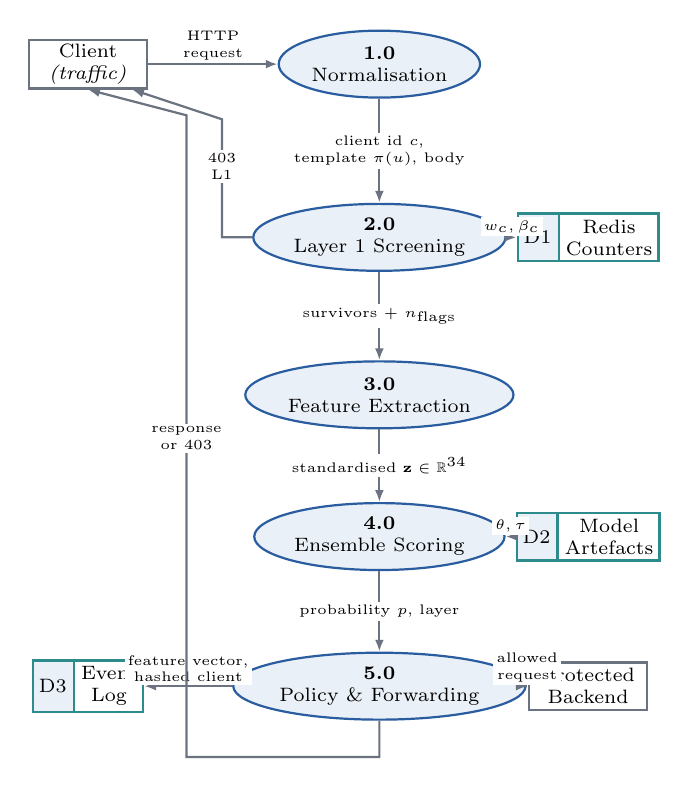
\begin{tikzpicture}[
  font=\scriptsize,
  ext/.style={draw=srGrey,thick,fill=white,minimum height=6mm,text width=14mm,
              align=center,inner sep=1.5pt},
  proc/.style={draw=srBlue,thick,fill=srLight,ellipse,align=center,inner sep=1.2pt,
               minimum width=25mm,minimum height=8.5mm},
  store/.style={draw=srTeal,thick,rectangle split,rectangle split parts=2,
                rectangle split horizontal,align=center,inner sep=2.2pt,
                rectangle split part fill={srLight,white}},
  fl/.style={-{Latex[length=1.5mm]},draw=srGrey,thick},
  lb/.style={font=\tiny,inner sep=1.2pt,fill=white,align=center}]

\node[ext]  (cli) at (-2.85, 0.15) {Client\\\textit{(traffic)}};
\node[proc] (p1)  at ( 0.85, 0.15) {\textbf{1.0}\\Normalisation};
\node[proc] (p2)  at ( 0.85,-2.05) {\textbf{2.0}\\Layer 1 Screening};
\node[proc] (p3)  at ( 0.85,-4.05) {\textbf{3.0}\\Feature Extraction};
\node[proc] (p4)  at ( 0.85,-5.85) {\textbf{4.0}\\Ensemble Scoring};
\node[proc] (p5)  at ( 0.85,-7.75) {\textbf{5.0}\\Policy \& Forwarding};

\node[store] (d1) at ( 3.50,-2.05) {D1 \nodepart{two} Redis\\Counters};
\node[store] (d2) at ( 3.50,-5.85) {D2 \nodepart{two} Model\\Artefacts};
\node[ext]   (be) at ( 3.50,-7.75) {Protected\\Backend};
\node[store] (d3) at (-2.85,-7.75) {D3 \nodepart{two} Event\\Log};

\draw[fl] (cli.east) -- node[lb,above]{HTTP\\request} (p1.west);
\draw[fl] (p1) -- node[lb]{client id $c$,\\template $\pi(u)$, body} (p2);
\draw[fl] (p2) -- node[lb]{survivors $+$ $n_{\text{flags}}$} (p3);
\draw[fl] (p3) -- node[lb]{standardised $\mathbf{z}\in\mathbb{R}^{34}$} (p4);
\draw[fl] (p4) -- node[lb]{probability $p$, layer} (p5);

\draw[fl] (p2.east) -- node[lb,above]{$w_c,\beta_c$} (d1.west);
\draw[fl] (d2.west) -- node[lb,above]{$\theta,\tau$} (p4.east);
\draw[fl] (p5.east) -- node[lb,above]{allowed\\request} (be.west);
\draw[fl] (p5.west) -- node[lb,above]{feature vector,\\hashed client} (d3.east);

\draw[fl] (p2.west) -- (-1.15,-2.05) -- (-1.15,-0.55) -- (cli.-30);
\node[lb] at (-1.15,-1.15) {403\\L1};
\draw[fl] (p5.south) -- (0.85,-8.65) -- (-1.60,-8.65) -- (-1.60,-0.50) -- (cli.south);
\node[lb] at (-1.60,-4.6) {response\\or 403};
\end{tikzpicture}
\caption{Level-1 data-flow diagram. Only process 5.0 reaches the protected backend, and only
with a request every prior stage has cleared. The event log stores feature vectors and hashed
client identifiers; raw bodies are never written.}
\label{fig:dfd}
\end{figure}

\begin{itemize}[leftmargin=1.2em,itemsep=1pt,topsep=2pt]
  \item \textbf{1.0 Normalisation} derives the client identifier, collapses the path to a
        template $\pi(u)$, and caps the body at 1\,MiB with the first 64\,KiB inspected.
  \item \textbf{2.0 Layer 1 Screening} applies 26 signature rules and the Redis sliding-window
        limiter. A blocking hit returns 403 immediately; advisory hits become a feature.
  \item \textbf{3.0 Feature Extraction} produces the 34-dimensional shape vector and
        standardises it against the baseline.
  \item \textbf{4.0 Ensemble Scoring} runs the isolation forest, the autoencoder and the
        meta-learner, producing one probability.
  \item \textbf{5.0 Policy and Forwarding} applies the operating mode, forwards or rejects,
        and appends to the event log.
  \item \textbf{Data stores.} D1 holds per-client counters; D2 holds the fitted models,
        baseline and threshold, mounted read-only; D3 is the append-only event log that feeds
        recalibration and retraining.
\end{itemize}

\subsection{Control-Flow View}
\label{sec:flow}
Fig.~\ref{fig:arch} shows the same system as an execution flow, adding what a data-flow
diagram omits: the sequential order of layers L1--L4 and the branches at which a request
terminates early.

\begin{figure}[t]
\centering
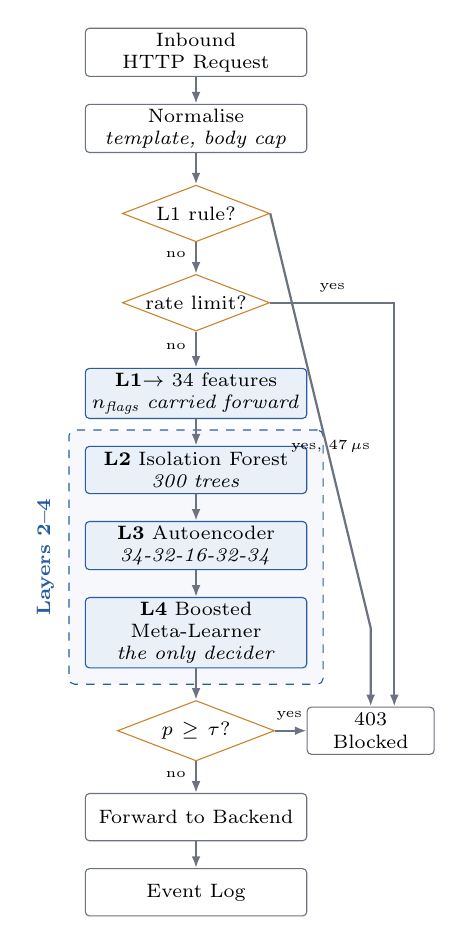
\begin{tikzpicture}[
  font=\scriptsize,
  node distance=3.4mm,
  box/.style={draw=srGrey,fill=white,rounded corners=1.5pt,minimum height=6.0mm,
              text width=27mm,align=center,inner sep=1.6pt},
  stage/.style={box,draw=srBlue,fill=srLight,text width=27mm},
  dec/.style={draw=srAmber,fill=white,diamond,aspect=2.6,inner sep=0.5pt,
              text width=13mm,align=center},
  ar/.style={-{Latex[length=1.5mm]},draw=srGrey,thick}]

\node[box] (cli) {Inbound HTTP Request};
\node[box,below=of cli] (norm) {Normalise\\\textit{template, body cap}};
\node[dec,below=4.0mm of norm] (r1) {L1 rule?};
\node[dec,below=4.0mm of r1] (r2) {rate limit?};

\node[stage,below=4.6mm of r2] (feat) {\textbf{L1$\rightarrow$} 34 features\\\textit{$n_{\text{flags}}$ carried forward}};
\node[stage,below=of feat] (l2) {\textbf{L2} Isolation Forest\\\textit{300 trees}};
\node[stage,below=of l2] (l3) {\textbf{L3} Autoencoder\\\textit{34-32-16-32-34}};
\node[stage,below=of l3] (l4) {\textbf{L4} Boosted Meta-Learner\\\textit{the only decider}};

\node[dec,below=4.0mm of l4] (thr) {$p\ge\tau$?};
\node[box,below=4.0mm of thr] (fwd) {Forward to Backend};
\node[box,right=4.0mm of thr,text width=15mm] (blk) {403\\Blocked};
\node[box,below=of fwd] (log) {Event Log};

\begin{scope}[on background layer]
  \node[draw=srBlue,dashed,rounded corners=2pt,inner sep=2.0mm,
        fit=(l2)(l3)(l4),fill=srLight!45] (ml) {};
\end{scope}
\node[srBlue,rotate=90,anchor=south,font=\scriptsize\bfseries]
     at ($(ml.west)+(-0.6mm,0)$) {Layers 2--4};

\draw[ar] (cli) -- (norm);
\draw[ar] (norm) -- (r1);
\draw[ar] (r1) -- node[left,pos=0.4,font=\tiny]{no} (r2);
\draw[ar] (r2) -- node[left,pos=0.4,font=\tiny]{no} (feat);
\draw[ar] (feat) -- (l2);
\draw[ar] (l2) -- (l3);
\draw[ar] (l3) -- (l4);
\draw[ar] (l4) -- (thr);
\draw[ar] (thr) -- node[left,pos=0.4,font=\tiny]{no} (fwd);
\draw[ar] (thr) -- node[above,pos=0.45,font=\tiny]{yes} (blk);
\draw[ar] (fwd) -- (log);
\draw[ar] (r1.east) -- node[above,pos=0.6,font=\tiny]{yes, 47\,$\mu$s} ($(blk.north)+(0,10mm)$) -- (blk.north);
\draw[ar] (r2.east) -| node[above,pos=0.25,font=\tiny]{yes} ($(blk.north)+(3mm,0)$);
\end{tikzpicture}
\caption{Control flow. The two early exits from L1 bypass every model, which is the mechanism
behind the $116\times$ latency gap between a rule verdict and a full evaluation.}
\label{fig:arch}
\end{figure}

%=============================================================================
\section{Methodology}
\label{sec:method}
\subsection{Formalisation}
Let a request be $r=(m,u,q,b,H,c,t)$ with method $m$, path $u$, query $q$, body $b$, headers
$H$, client identifier $c$ and arrival time $t$. The gateway computes
$\mathcal{D}(r)\in\{\textsc{allow},\textsc{block}\}$ before forwarding. A template map $\pi$
collapses variable path segments, so
$\pi(\texttt{/orders/8813})=\texttt{/orders/\{id\}}$ and per-endpoint statistics aggregate
across identifier values.

A feature map $\phi:\mathcal{R}\rightarrow\mathbb{R}^{d}$, $d=34$, yields
$\mathbf{x}=\phi(r)$, standardised against the normal-only pool $\mathcal{B}$:
\begin{equation}
\mathbf{z}=\frac{\mathbf{x}-\boldsymbol{\mu}_{\mathcal{B}}}
{\boldsymbol{\sigma}_{\mathcal{B}}},\qquad
\boldsymbol{\mu}_{\mathcal{B}},\boldsymbol{\sigma}_{\mathcal{B}}\in\mathbb{R}^{34}.
\label{eq:standardise}
\end{equation}
Critically, $\phi$ encodes request \emph{shape} and never route identity
(Table~\ref{tab:features}). An earlier iteration admitting endpoint identity degenerated into
a lookup table that memorised which routes had been attacked in training; $\pi(u)$ therefore
keys baselines only and never reaches a model. Three features are baseline-relative: for raw
value $v$ with reference $(\mu,\sigma)$,
\begin{equation}
z_{\text{rel}}(v)=
\begin{cases}
(v-\mu)/\sigma, & \sigma > \varepsilon\\
0, & \text{otherwise,}
\end{cases}
\qquad \varepsilon=10^{-9}.
\label{eq:relz}
\end{equation}

\begin{table}[H]
\caption{Feature Vector Composition, $d=34$}
\label{tab:features}
\centering
\footnotesize
\begin{tabularx}{\columnwidth}{@{}rlL@{}}
\toprule
$n$ & \textbf{Group} & \textbf{Captures} \\
\midrule
7  & Body shape   & Size, Shannon entropy, character-class ratios; one baseline-relative $z$ \\
2  & Content      & Body presence, declared JSON type \\
11 & Path shape   & Length, depth, entropy, class ratios, dot count, raw/decoded delta \\
5  & Query        & Parameter count, value lengths, special ratio, decode delta \\
1  & Behaviour    & Distinct templates in the client window \\
7  & Method       & One-hot HTTP method plus write indicator \\
1  & L1 evidence  & Advisory rule-hit count $n_{\text{flags}}$ \\
\bottomrule
\end{tabularx}
\end{table}

\subsection{Layer 1: Deterministic Screening}
Let $\mathcal{S}$ be 26 compiled signature rules partitioned into $\mathcal{S}_{b}$
($|\mathcal{S}_b|=22$, blocking) and $\mathcal{S}_{f}$ ($|\mathcal{S}_f|=4$, advisory),
covering SQL injection, cross-site scripting, traversal, command injection, scanning,
server-side template injection, deserialisation and SSRF. Writing $\mathcal{S}(r)$ for the
rules that match, a request is rejected when
$\mathcal{S}_b\cap\mathcal{S}(r)\neq\emptyset$. Advisory hits do not decide; their count
$n_{\text{flags}}=|\mathcal{S}_f\cap\mathcal{S}(r)|$ enters $\phi$, so weak signature evidence
informs the model rather than overriding it.

Redis maintains per client a window count $w_c$ over $W_{\text{win}}=60$\,s, a burst count
$\beta_c$ over $W_{\text{burst}}=5$\,s, and a HyperLogLog cardinality of templates touched, in
one pipeline of 11 commands. The rate verdict is
\begin{equation}
\text{limited}(c)\iff \beta_c>\Lambda_{\beta}\ \vee\ w_c>\Lambda_{w},
\label{eq:rate}
\end{equation}
with $\Lambda_{\beta}=40$ and $\Lambda_{w}=240$.

\subsection{Layers 2--4: The Stacking Ensemble}
Layer~2 is an isolation forest of $T=300$ trees over subsample $\psi=3695$. For a point
$\mathbf{z}$ with expected path length $\mathbb{E}[h(\mathbf{z})]$,
\begin{equation}
s_{\text{IF}}(\mathbf{z})=2^{-\mathbb{E}[h(\mathbf{z})]/c(\psi)},\ \
c(\psi)=2\!\left(\ln(\psi{-}1)+\gamma\right)-\tfrac{2(\psi-1)}{\psi},
\label{eq:iforest}
\end{equation}
$\gamma$ the Euler--Mascheroni constant. Layer~3 is a fully connected autoencoder
$34\!\rightarrow\!32\!\rightarrow\!16\!\rightarrow\!32\!\rightarrow\!34$ with $3{,}314$
trainable parameters, implemented directly in NumPy. With encoder $f_{\theta}$ and decoder
$g_{\vartheta}$,
\begin{equation}
\hat{\mathbf{z}}=g_{\vartheta}(f_{\theta}(\mathbf{z})),\qquad
s_{\text{AE}}(\mathbf{z})=\lVert\mathbf{z}-\hat{\mathbf{z}}\rVert_{2}^{2},
\label{eq:ae}
\end{equation}
trained by minimising $s_{\text{AE}}$ over $\mathcal{B}$ with Adam, $\eta=10^{-3}$, batch
256 and early-stopping patience 15. Avoiding a deep-learning framework removes a
$\sim$2\,GB dependency and holds inference to 30\,$\mu$s.

Both scores are min--max mapped with bounds fitted at training time,
\begin{equation}
\tilde{s}=\min\!\left(1,\max\!\left(0,
\frac{s-s_{\text{lo}}}{s_{\text{hi}}-s_{\text{lo}}+\varepsilon}\right)\right),
\label{eq:norm}
\end{equation}
and a third input summarises rate pressure, $s_{\text{rate}}=\min(1,w_c/\Lambda_w)$. Layer~4
is a histogram-based gradient boosting classifier $g$ of $M=107$ boosting iterations:
\begin{equation}
p=g\!\left(s_{\text{rate}},\tilde{s}_{\text{IF}},\tilde{s}_{\text{AE}}\right)\in[0,1].
\label{eq:meta}
\end{equation}
The complete decision is
\begin{equation}
\mathcal{D}(r)=
\begin{cases}
\textsc{block}, & \mathcal{S}_b\cap\mathcal{S}(r)\neq\emptyset\\
\textsc{block}, & \text{limited}(c)\\
\textsc{block}, & p\ge\tau\ \wedge\ \text{mode}=\texttt{enforce}\\
\textsc{allow}, & \text{otherwise.}
\end{cases}
\label{eq:decision}
\end{equation}

Base detectors are fitted only on $\mathcal{B}$ and the meta-learner on a disjoint pool
$\mathcal{M}$, so meta-features are out-of-sample by construction and no $k$-fold out-of-fold
stacking procedure is required.

Algorithm~\ref{alg:inspect} states the request path. The early returns at lines~3 and~6 are
the mechanism behind the $116\times$ latency gap: a blocking rule hit never reaches
\eqref{eq:iforest}.

\begin{algorithm}[H]
\SetAlgoLined
\KwIn{request $r$; models $(\mathcal{S},\text{IF},\text{AE},g)$; baseline $\mathcal{B}$;
      threshold $\tau$}
\KwOut{verdict, deciding layer, probability}
$u \leftarrow \pi(\textrm{path}(r))$;\ \ $b \leftarrow$ first $2^{16}$ bytes of body
  \tcp*{1\,MiB hard cap}
$\mathcal{H} \leftarrow \mathcal{S}(r)$ \tcp*{26 compiled rules}
\lIf{$\mathcal{S}_b\cap\mathcal{H}\neq\emptyset$}
  {\Return $(\textsc{block},\textsc{l1-rules},1.0)$}
$(w_c,\beta_c,\cdot) \leftarrow \textsc{RedisPipeline}(c,u)$ \tcp*{11 commands}
\lIf{$\textrm{limited}(c)$ by \eqref{eq:rate}}
  {\Return $(\textsc{block},\textsc{l1-rate},1.0)$}
$n_{\text{flags}} \leftarrow |\mathcal{S}_f\cap\mathcal{H}|$\;
$\mathbf{z} \leftarrow$ standardise $\phi(r,n_{\text{flags}})$ by \eqref{eq:standardise}\;
$\tilde{s}_{\text{IF}} \leftarrow$ normalise \eqref{eq:iforest};\ \
$\tilde{s}_{\text{AE}} \leftarrow$ normalise \eqref{eq:ae}\;
$s_{\text{rate}} \leftarrow \min(1,\,w_c/\Lambda_w)$\;
$p \leftarrow g(s_{\text{rate}},\tilde{s}_{\text{IF}},\tilde{s}_{\text{AE}})$\;
\lIf{$p \ge \tau$}{\Return $(\textsc{block},\textsc{l4-meta},p)$}
\Return $(\textsc{allow},\varnothing,p)$\;
\caption{Request-time inspection}
\label{alg:inspect}
\end{algorithm}

\subsection{Graded Enforcement}
Three modes select which layers may act on \eqref{eq:decision}: \texttt{monitor} (log only),
\texttt{enforce-l1} (default; L1 blocks, L4 logs) and \texttt{enforce} (all block). The
gradation is empirical. Layer~1 is deterministic and produced no false positives in our
evaluation, whereas a model fitted on our corpus and exposed to a different client population
produced a 13.6\% false-positive rate even after threshold recalibration.

\subsection{Calibration to an Unseen Backend}
Porting to a new backend changes only the upstream URL. Adaptation re-derives
$(\boldsymbol{\mu}_{\mathcal{B}},\boldsymbol{\sigma}_{\mathcal{B}})$ and $\tau$ from a
monitor-mode window and updates no weights: fine-tuning on a short window invites catastrophic
forgetting, and any online weight update is a poisoning surface for an adversary generating
traffic during that window. Algorithm~\ref{alg:calib} states the four numeric gates that abort
calibration rather than emit an unsafe threshold.

\begin{algorithm}[H]
\SetAlgoLined
\KwIn{monitor window $\mathcal{W}$; budget $\alpha=0.01$; $N_{\min}=2000$; $\kappa=0.02$}
\KwOut{updated $(\boldsymbol{\mu},\boldsymbol{\sigma},\tau)$ or \textsc{abort}}
\lIf{$|\mathcal{W}|<N_{\min}$}{\Return \textsc{abort}}
$\mathcal{W}_c \leftarrow \{\,r\in\mathcal{W} : \mathcal{S}_b\cap\mathcal{S}(r)=\emptyset\,\}$\;
\lIf{$1-|\mathcal{W}_c|/|\mathcal{W}| > \kappa$}{\Return \textsc{abort}}
recompute $(\boldsymbol{\mu},\boldsymbol{\sigma})$ over $\mathcal{W}_c$; refresh
\eqref{eq:relz}\;
$P \leftarrow \{\,g(\cdot)\ \textrm{for}\ r\in\mathcal{W}_c\,\}$
  \tcp*{existing models, no refit}
\lIf{$\mathrm{median}(P)\ge 0.5$}{\Return \textsc{abort}}
$\tau' \leftarrow \mathrm{Quantile}(P,\,1-\alpha)$\;
\lIf{$\tau'<0.2 \ \vee\ \tau'-\tau>0.3$}{\Return \textsc{abort}}
\Return $(\boldsymbol{\mu},\boldsymbol{\sigma},\tau')$\;
\caption{Calibration with admission gates}
\label{alg:calib}
\end{algorithm}

\subsection{Complexity and Expected Cost}
\label{sec:complexity}
Let $|r|$ be inspected bytes, $R=|\mathcal{S}|=26$, $T=300$, $\psi=3695$, $M=107$ and
$\{d_i\}=\{34,32,16,32,34\}$. Per request,
\begin{align}
C_{\text{L1}} &= O(R\,|r|), & C_{\text{L2}} &= O(T\log\psi),\\
C_{\text{L3}} &= O\!\Big(\textstyle\sum_{i=1}^{3} d_i d_{i+1}\Big)=3{,}314\ \text{MACs},
& C_{\text{L4}} &= O(M).
\end{align}
Because Layer~1 short-circuits, expected cost depends on traffic composition:
\begin{equation}
\mathbb{E}[C]=\rho\,C_{\text{L1}}+(1-\rho)\!
\left(C_{\text{L1}}+C_{\text{L2}}+C_{\text{L3}}+C_{\text{L4}}\right),
\label{eq:expcost}
\end{equation}
with $\rho$ the fraction settled deterministically. At $\rho=0.30$ the mean falls from
5.43\,ms to 3.82\,ms.

\subsection{Evaluation Protocol}
\label{sec:protocol}
Requests are assigned to pools by hashing the client identifier with seed $\sigma$, never the
row:
\begin{equation}
\text{pool}(c)=\Pi\!\left[\,\mathcal{H}(c\Vert\sigma)\bmod 100\,\right],\
\Pi:\{0..99\}\rightarrow\{\mathcal{B},\mathcal{M},\mathcal{V},\mathcal{T}\}.
\label{eq:pool}
\end{equation}
Row-level splitting lets near-identical requests from one session straddle the boundary and
inflates every metric. Families $\{\texttt{cmdi},\texttt{exfil},\texttt{ssti}\}$ occur only in
$\mathcal{T}$, following \cite{alam2025adaptive}; zero-day recall is measured solely on them.
The threshold is fixed on validation under an explicit budget,
\begin{equation}
\tau=\min\{t\in[0,1]:\mathrm{FPR}_{\mathcal{V}}(t)\le\alpha\},\qquad \alpha=0.01,
\label{eq:tau}
\end{equation}
giving $\tau=0.25$. Every baseline receives the same budget, otherwise the comparison rewards
whichever model was permitted to be loosest. $\mathcal{T}$ is read once. Requests stopped by
L1 are excluded from model scoring and re-attached for the end-to-end figure, since in
deployment they never reach a model.

%=============================================================================
\section{Results and Discussion}
\label{sec:results}
\subsection{Input Data and How a Result Is Produced}
\label{sec:inputs}
A standard-library simulator drove a FastAPI backend with the gateway in monitor mode, so
attacks appear in the log rather than terminating at a 403. The corpus holds $14{,}960$
labelled requests from $1{,}061$ client sessions over $1{,}503$ endpoint templates:
$9{,}224$ normal (61.7\%) and $5{,}641$ attack (37.7\%). Table~\ref{tab:corpus} gives the
family breakdown. Labels exist only because a laboratory flag admits a ground-truth header;
that flag is a training-data poisoning channel and is rejected in production configurations.

\begin{table}[H]
\caption{Corpus Composition ($^{*}$ withheld from all pools but test)}
\label{tab:corpus}
\centering
\footnotesize
\begin{tabularx}{\columnwidth}{@{}LrLr@{}}
\toprule
\textbf{Family} & \textbf{$n$} & \textbf{Family} & \textbf{$n$} \\
\midrule
flood       & 1{,}981 & traversal & 48 \\
exfil$^{*}$ & 1{,}669 & cmdi$^{*}$ & 37 \\
bruteforce  & 1{,}419 & payload   & 19 \\
scan        & 314     & ssti$^{*}$ & 13 \\
sqli        & 80      & \textbf{normal} & \textbf{9{,}224} \\
xss         & 61      & \textbf{total}  & \textbf{14{,}960} \\
\bottomrule
\end{tabularx}
\end{table}

For the reported seed the pools hold $|\mathcal{B}|=3695$, $|\mathcal{M}|=3611$,
$|\mathcal{V}|=2031$ and $|\mathcal{T}|=2127$. One evaluation record is a request with its
ground-truth family; the detector sees only the request. Per-record verdicts are aggregated
into the metrics of Tables~\ref{tab:seeds}--\ref{tab:abl}.

\subsection{Per-Seed Behaviour}
\label{sec:seeds}
Table~\ref{tab:seeds} reports all ten partitions and Fig.~\ref{fig:seeds} plots them. Because
each seed induces a different session partition via \eqref{eq:pool}, the spread measures
sensitivity to \emph{which clients} land in which pool---the dominant variance source in a
session-grouped design.

\begin{table}[H]
\caption{Per-Seed Results Over Ten Session Partitions}
\label{tab:seeds}
\centering
\footnotesize
\setlength{\tabcolsep}{4pt}
\begin{tabularx}{\columnwidth}{@{}Lrrrrr@{}}
\toprule
\textbf{Seed} & \textbf{Prec.} & \textbf{Rec.} & \textbf{$F_1$} & \textbf{FPR} &
\textbf{Zero-day} \\
\midrule
1  & 0.9850 & 0.8748 & 0.9266 & 0.0081 & 0.4261 \\
2  & 0.9961 & 0.9898 & 0.9929 & 0.0023 & 0.9971 \\
3  & 0.9699 & 0.8724 & 0.9186 & 0.0138 & 0.5122 \\
4  & 0.9881 & 0.9371 & 0.9619 & 0.0065 & 0.8794 \\
5  & 0.9876 & 0.9958 & 0.9917 & 0.0061 & 0.9896 \\
6  & 0.9866 & 0.8596 & 0.9188 & 0.0054 & 0.5907 \\
7  & 0.9835 & 0.9755 & 0.9795 & 0.0086 & 0.9283 \\
8  & 0.9928 & 0.9050 & 0.9469 & 0.0035 & 0.8645 \\
9  & 0.9881 & 0.9989 & 0.9935 & 0.0079 & 1.0000 \\
10 & 0.9847 & 0.9059 & 0.9437 & 0.0072 & 0.7546 \\
\midrule
\textbf{mean} & 0.9862 & 0.9315 & 0.9574 & 0.0069 & 0.7943 \\
\textbf{sd}   & 0.0069 & 0.0551 & 0.0307 & 0.0031 & \textbf{0.2134} \\
\bottomrule
\end{tabularx}
\end{table}

\begin{figure}[t]
\centering
\resizebox{\columnwidth}{!}{%
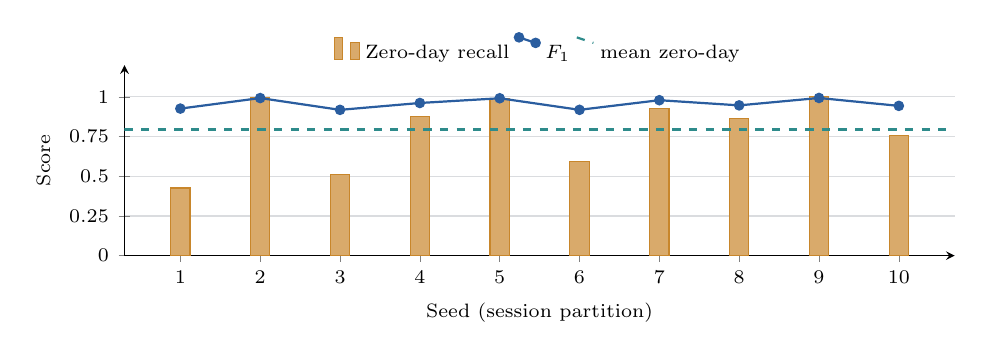
\begin{tikzpicture}
\begin{axis}[
  width=\columnwidth, height=4.0cm,
  ybar, bar width=7pt,
  xtick={1,...,10}, xmin=0.3, xmax=10.7, ymin=0, ymax=1.20,
  ytick={0,0.25,0.5,0.75,1.0},
  ylabel={Score}, xlabel={Seed (session partition)},
  ylabel near ticks, xlabel near ticks,
  xticklabel style={font=\scriptsize}, yticklabel style={font=\scriptsize},
  label style={font=\scriptsize},
  legend style={font=\scriptsize,at={(0.5,1.20)},anchor=north,legend columns=3,draw=none},
  ymajorgrids, grid style={srGrey!25}, axis lines=left]
\addplot[fill=srAmber!70,draw=srAmber] coordinates
  {(1,0.4261) (2,0.9971) (3,0.5122) (4,0.8794) (5,0.9896)
   (6,0.5907) (7,0.9283) (8,0.8645) (9,1.0000) (10,0.7546)};
\addplot[srBlue,thick,mark=*,mark size=1.5pt,sharp plot] coordinates
  {(1,0.9266) (2,0.9929) (3,0.9186) (4,0.9619) (5,0.9917)
   (6,0.9188) (7,0.9795) (8,0.9469) (9,0.9935) (10,0.9437)};
\addplot[srTeal,thick,dashed,sharp plot] coordinates {(0.3,0.7943) (10.7,0.7943)};
\legend{Zero-day recall,$F_1$,mean zero-day}
\end{axis}
\end{tikzpicture}}
\caption{Per-seed zero-day recall against $F_1$. $F_1$ is stable (sd $0.031$); zero-day recall
ranges $0.426$--$1.000$ (sd $0.213$) with the key graph and every hyperparameter fixed.}
\label{fig:seeds}
\end{figure}

Precision is high and stable (sd $0.0069$) and FPR sits inside the 1\% budget on 9 of 10
seeds. Zero-day recall is the outlier at sd $0.2134$, some $31\times$ the precision spread.
That spread is the most informative number in the paper. With three withheld families and
session-grouped splits, whether a seed places diverse exfiltration sessions in $\mathcal{T}$
moves the result by more than half its range. Reporting seed~9 alone would let us claim
zero-day recall $1.000$---real, reproducible, and misleading. Table~\ref{tab:main} gives the
intervals we report instead.

\begin{table}[H]
\caption{Ten-Seed Summary, Mean With 95\% Confidence Interval}
\label{tab:main}
\centering
\footnotesize
\begin{tabularx}{\columnwidth}{@{}Lrcr@{}}
\toprule
\textbf{Metric} & \textbf{Mean} & \textbf{95\% CI} & \textbf{Range} \\
\midrule
$F_1$           & 0.9574 & $[0.9398,\,0.9756]$ & 0.919--0.994 \\
Precision       & 0.9862 & $[0.9818,\,0.9900]$ & 0.970--0.996 \\
Recall          & 0.9315 & $[0.8997,\,0.9642]$ & 0.860--0.999 \\
FPR             & 0.0069 & $[0.0052,\,0.0089]$ & 0.002--0.014 \\
ROC AUC         & 0.9894 & $[0.9717,\,0.9991]$ & 0.911--1.000 \\
PR AUC          & 0.9888 & $[0.9729,\,0.9980]$ & 0.921--1.000 \\
Zero-day recall & 0.7943 & $[0.6679,\,0.9137]$ & \textbf{0.426--1.000} \\
\bottomrule
\end{tabularx}
\end{table}

\subsection{Ablation and Significance}
Table~\ref{tab:ablation} compares each detector alone against the stack on identical test
requests under a common budget, and Fig.~\ref{fig:ablation} plots it. McNemar's test on paired
predictions uses
\begin{equation}
\chi^{2}=\frac{\left(|n_{01}-n_{10}|-1\right)^{2}}{n_{01}+n_{10}},
\label{eq:mcnemar}
\end{equation}
where $n_{01}$ counts requests the stack classifies correctly and the baseline does not.

\begin{table}[H]
\caption{Ablation on Identical Test Requests, With McNemar Against the Stack}
\label{tab:ablation}
\centering
\footnotesize
\setlength{\tabcolsep}{4pt}
\begin{tabularx}{\columnwidth}{@{}Lrrrrrr@{}}
\toprule
\textbf{Detector} & \textbf{Prec.} & \textbf{Rec.} & \textbf{$F_1$} &
\textbf{$n_{01}$} & \textbf{$n_{10}$} & \textbf{$\chi^2$} \\
\midrule
Rate signal      & 0.981 & 0.349 & 0.515 & 488 & 13 & 448.5 \\
Isolation Forest & 0.875 & 0.264 & 0.406 & 565 & 4  & 551.1 \\
Autoencoder      & 0.983 & 0.780 & 0.870 & 163 & 3  & 152.3 \\
\textbf{Stack}   & \textbf{0.983} & \textbf{1.000} & \textbf{0.991} & --- & --- & --- \\
\bottomrule
\end{tabularx}
\end{table}

\begin{figure}[t]
\centering
\resizebox{\columnwidth}{!}{%
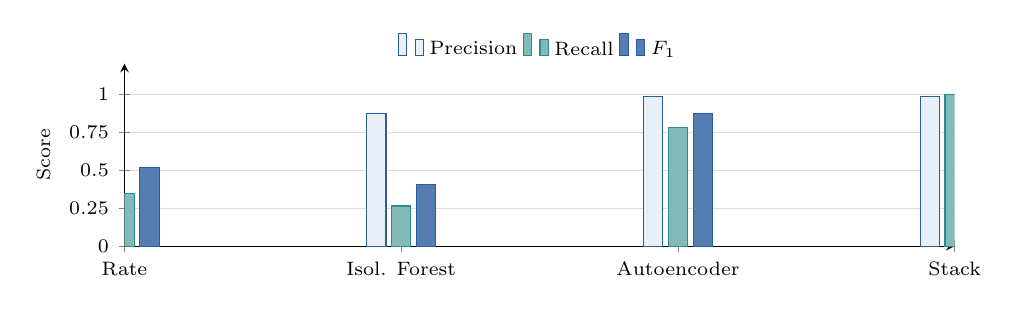
\begin{tikzpicture}
\begin{axis}[
  width=\columnwidth, height=3.9cm,
  ybar, bar width=7pt,
  symbolic x coords={Rate,Isol. Forest,Autoencoder,Stack},
  xtick=data, ymin=0, ymax=1.20, ytick={0,0.25,0.5,0.75,1.0},
  enlarge x limits=0.16,
  ylabel={Score}, ylabel near ticks,
  xticklabel style={font=\scriptsize}, yticklabel style={font=\scriptsize},
  label style={font=\scriptsize},
  legend style={font=\scriptsize,at={(0.5,1.20)},anchor=north,legend columns=3,draw=none},
  ymajorgrids, grid style={srGrey!25}, axis lines=left]
\addplot[fill=srLight,draw=srBlue] coordinates
  {(Rate,0.981) (Isol. Forest,0.875) (Autoencoder,0.983) (Stack,0.983)};
\addplot[fill=srTeal!60,draw=srTeal] coordinates
  {(Rate,0.349) (Isol. Forest,0.264) (Autoencoder,0.780) (Stack,1.000)};
\addplot[fill=srBlue!80,draw=srBlue] coordinates
  {(Rate,0.515) (Isol. Forest,0.406) (Autoencoder,0.870) (Stack,0.991)};
\legend{Precision,Recall,$F_1$}
\end{axis}
\end{tikzpicture}}
\caption{Every constituent detector against the stack on identical test requests. Precision is
uniformly high; the ensemble's gain is almost entirely in recall.}
\label{fig:ablation}
\end{figure}

The autoencoder dominates individually; the isolation forest alone recalls only 26.4\% of
attacks. All three improvements are significant at $\chi^2\ge152.3$, $p<10^{-34}$. Two caveats
bind Table~\ref{tab:ablation}: it is a single partition, and the recall of $1.000$ is a
property of that partition, not a general claim---the defensible figure remains
$0.9315\ [0.8997,0.9642]$. The comparison harness also rebuilds each model independently so
all four score identical rows, as McNemar's pairing assumption requires, but does not inherit
every hyperparameter from the deployed artefact; magnitudes are indicative and the ranking is
robust.

\subsection{The Fused Boundary Is Non-Monotonic}
\label{sec:nonmono}
Across all L1-clean corpus rows, both base scores are positively associated with the attack
label: the isolation forest attains AUC $0.831$ (mean $0.240$ on normal against $0.550$ on
attack) and the autoencoder AUC $0.980$. Globally, higher means more anomalous.

The fused surface is not monotone in that direction everywhere. Evaluating \eqref{eq:meta}
over a grid at $s_{\text{rate}}=0.004$ (Table~\ref{tab:surface}) shows that at
$\tilde{s}_{\text{AE}}=0.25$ the output falls from $p=0.999$ at
$\tilde{s}_{\text{IF}}=0.00$ to $p=0.004$ at $\tilde{s}_{\text{IF}}=1.00$: over this slice a
\emph{higher} isolation-forest score makes an attack verdict \emph{less} likely.

\begin{table}[H]
\caption{Meta-Learner Output $p$ Over the Fused Input Grid, $s_{\text{rate}}=0.004$}
\label{tab:surface}
\centering
\footnotesize
\setlength{\tabcolsep}{5pt}
\begin{tabularx}{\columnwidth}{@{}Lrrrrr@{}}
\toprule
$\tilde{s}_{\text{IF}}\ \backslash\ \tilde{s}_{\text{AE}}$
 & \textbf{0.00} & \textbf{0.25} & \textbf{0.50} & \textbf{0.75} & \textbf{1.00} \\
\midrule
0.00 & 0.000 & 0.999 & 0.999 & 1.000 & 1.000 \\
0.25 & 0.000 & 0.998 & 0.998 & 1.000 & 1.000 \\
0.50 & 0.000 & 0.024 & 0.024 & 0.128 & 0.976 \\
0.75 & 0.000 & 0.007 & 0.007 & 0.025 & 0.739 \\
1.00 & 0.000 & 0.004 & 0.004 & 0.013 & 0.636 \\
\bottomrule
\end{tabularx}
\end{table}

This explains the motivating case of Section~\ref{sec:case} exactly, and it explains the
meta-learner search result. A search on seeds $\{11..15\}$, disjoint from the reporting seeds
and with the pseudo-novel triple $\{\texttt{bruteforce},\texttt{scan},\texttt{flood}\}$ so the
real withheld families never informed a hyperparameter, favoured gradient boosting decisively
(Table~\ref{tab:abl}): objective $0.884$ against $0.744$, driven almost entirely by validation
$F_1$ ($0.943$ against $0.668$, a $+0.275$ absolute gain) since pseudo zero-day recall barely
moves ($0.826$ against $0.820$). A linear meta-learner cannot represent the region in
Table~\ref{tab:surface} at all.

We report this rather than presenting the gain as unqualified progress. A boundary with
locally inverted polarity is fitted tightly to the training population, and is a plausible
contributor to the 13.6\% false-positive rate observed when the model met a different client
population. Recall-only reporting would have hidden the entire phenomenon.

\subsection{Cost}
Table~\ref{tab:latency} pairs the complexity of Section~\ref{sec:complexity} with measurement,
single-threaded over 2{,}000 iterations after warm-up, and Fig.~\ref{fig:latency} plots it.

\begin{table}[H]
\caption{Per-Request Cost: Complexity and Measurement}
\label{tab:latency}
\centering
\footnotesize
\setlength{\tabcolsep}{4pt}
\begin{tabularx}{\columnwidth}{@{}LLrrr@{}}
\toprule
\textbf{Stage} & \textbf{Complexity} & \textbf{Mean} & \textbf{p50} & \textbf{p95} \\
\midrule
L1 rule block   & $O(R|r|)$        & 47\,$\mu$s & 48\,$\mu$s & 57\,$\mu$s \\
L2 isol. forest & $O(T\log\psi)$   & 3.37\,ms   & 3.20\,ms   & 4.33\,ms \\
L3 autoencoder  & 3{,}314 MACs     & 30\,$\mu$s & 25\,$\mu$s & 57\,$\mu$s \\
L4 meta-learner & $O(M)$, $M{=}107$& 1.44\,ms   & 1.30\,ms   & 2.11\,ms \\
\midrule
\textbf{Full ML path} & ---        & \textbf{5.43\,ms} & 5.06\,ms & 7.48\,ms \\
\bottomrule
\end{tabularx}
\end{table}

\begin{figure}[t]
\centering
\resizebox{\columnwidth}{!}{%
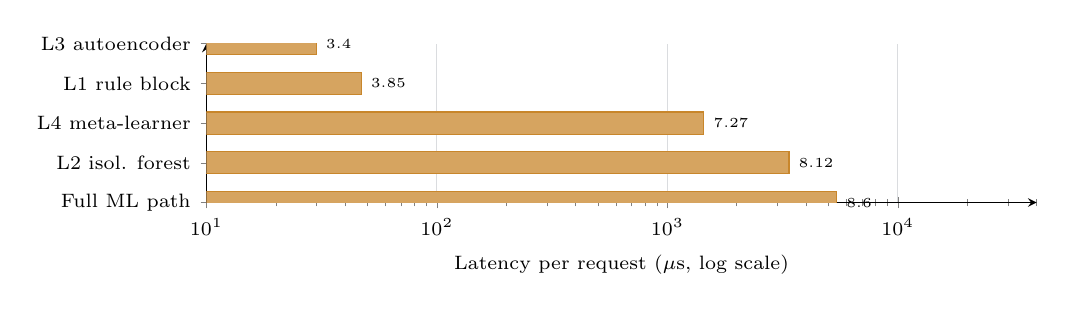
\begin{tikzpicture}
\begin{axis}[
  width=\columnwidth, height=3.6cm,
  xbar, bar width=8pt,
  xmode=log, xmin=10, xmax=40000,
  ytick={0,1,2,3,4},
  yticklabels={Full ML path,L2 isol. forest,L4 meta-learner,L1 rule block,L3 autoencoder},
  xlabel={Latency per request ($\mu$s, log scale)}, xlabel near ticks,
  xticklabel style={font=\scriptsize}, yticklabel style={font=\scriptsize},
  label style={font=\scriptsize},
  nodes near coords, every node near coord/.append style={font=\tiny},
  xmajorgrids, grid style={srGrey!25}, axis lines=left]
\addplot[fill=srAmber!75,draw=srAmber] coordinates
  {(5430,0) (3370,1) (1440,2) (47,3) (30,4)};
\end{axis}
\end{tikzpicture}}
\caption{Measured stage latency. The autoencoder is both the strongest single detector and the
cheapest stage; the isolation forest is the weakest detector and 62\% of the budget.}
\label{fig:latency}
\end{figure}

The ordering is counter-intuitive and actionable: the isolation forest costs 62\% of the
budget while contributing the least individually, so it is the first candidate for reduction
in a throughput-constrained deployment. By \eqref{eq:expcost}, cost also falls with the
hostile fraction of traffic, because attacks that trip a rule are rejected $116\times$ faster
than a clean request is cleared.

\subsection{Ablations}
Table~\ref{tab:abl} isolates the two design choices that are not inherited from prior work.

\begin{table}[H]
\caption{Meta-Learner Ablation on the Tuning Seeds}
\label{tab:abl}
\centering
\footnotesize
\begin{tabularx}{\columnwidth}{@{}Lrrr@{}}
\toprule
\textbf{Setting} & \textbf{$F_1$} & \textbf{Pseudo zero-day} & \textbf{Objective} \\
\midrule
\textbf{boosted meta-learner} & \textbf{0.943} & \textbf{0.826} & \textbf{0.884} \\
linear meta-learner           & 0.668 & 0.820 & 0.744 \\
\bottomrule
\multicolumn{4}{@{}l@{}}{\footnotesize Tuning seeds $\{11..15\}$ with a rotated pseudo-novel}\\
\multicolumn{4}{@{}l@{}}{\footnotesize family triple; objective $=0.5F_1+0.5$\,zero-day.}
\end{tabularx}
\end{table}

\subsection{Comparison With Prior Systems}
Table~\ref{tab:cmp} positions MicroAPI Guard against representative prior work. The comparison
is deliberately qualitative on capability rather than a leaderboard of scores, because those
scores are measured on different datasets under different supervision budgets and are not
directly comparable.

\begin{table}[H]
\caption{Capability Comparison With Prior Systems}
\label{tab:cmp}
\centering
\footnotesize
\setlength{\tabcolsep}{4pt}
\begin{tabularx}{\columnwidth}{@{}Lccccc@{}}
\toprule
\textbf{System} & \textbf{Inline} & \textbf{No} & \textbf{Latency} & \textbf{Withheld} &
\textbf{Interval} \\
 & \textbf{block} & \textbf{GPU} & \textbf{rep.} & \textbf{families} & \textbf{rep.} \\
\midrule
Auto-IF \cite{sadaf2020autoif}          & no  & yes & no  & no  & no \\
Jin et al. \cite{jin2020rpca}           & no  & yes & no  & no  & no \\
TraceAnomaly \cite{liu2020traceanomaly} & no  & no  & no  & no  & no \\
Al-Shehari \cite{alshehari2023insider}  & no  & yes & no  & no  & no \\
Sowmya \cite{sowmya2023api}             & yes & yes & no  & no  & no \\
LMGD \cite{liu2024lmgd}                 & no  & no  & no  & no  & no \\
DSEM-NIDS \cite{mahmoud2025dsem}        & no  & no  & no  & no  & no \\
Adaptive Def. \cite{alam2025adaptive}   & no  & no  & no  & yes & no \\
ART-FL \cite{raeiszadeh2025artfl}       & no  & no  & no  & no  & no \\
ADmM \cite{zhang2026admm}               & no  & no  & no  & no  & no \\
Huang \cite{huang2026gateway}           & near& yes & no  & no  & no \\
MRG \cite{levi2026mrg}                  & yes & no  & partial & no & no \\
\textbf{MicroAPI Guard (ours)} & \textbf{yes} & \textbf{yes} & \textbf{yes} &
\textbf{yes} & \textbf{yes} \\
\bottomrule
\end{tabularx}
\end{table}

Three columns matter most. \emph{Inline block} marks systems that refuse a request before it
reaches the backend rather than diagnosing it afterwards. \emph{Latency rep.} marks systems
publishing per-request detection cost beside accuracy; to our knowledge only MRG
\cite{levi2026mrg} reports anything comparable, and then only as a relative speedup.
\emph{Interval rep.} marks systems reporting confidence intervals over repeated partitions
rather than a point estimate---the reporting gap this paper closes.

\subsection{Reproducibility}
The system carries 102 assertion-based tests covering feature extraction, rule evaluation,
rate limiting and detector loading. The feature contract is enforced at load time: the gateway
refuses to start if the feature names recorded in the model artefact disagree with the running
code, making train/serve drift a startup failure rather than a silent accuracy loss. Every
number in this section is regenerated from the committed model artefacts.

\subsection{Limitations}
\textbf{Synthetic traffic.} The corpus is simulator-generated. The 13.6\% false-positive rate
measured on a different client population is direct evidence that cross-population
generalisation is unproven, and Section~\ref{sec:nonmono} identifies a plausible mechanism.

\textbf{Throughput unmeasured.} All latency figures are at concurrency one.
Equation~\eqref{eq:expcost} implies a ceiling near $184$ requests per second per core, but we
report no load test or tail latency under contention.

\textbf{Single deployment.} Portability follows from Algorithm~\ref{alg:calib}, not from an
experiment against an independently built backend.

\textbf{Ablation breadth.} The row-split control in Table~\ref{tab:abl} was not run, so the
inflation attributable to row-level splitting is argued rather than measured.

\textbf{Evasion.} We did not evaluate an adaptive adversary. Features built on character-class
ratios and encoding deltas are plausibly evadable by an attacker who shapes payloads
accordingly.

%=============================================================================
\section{Conclusion}
\label{sec:concl}
This paper presented MicroAPI Guard, a backend-agnostic API security gateway that screens
every request through 26 signature rules and a sliding-window rate limiter, and scores the
survivors with an isolation forest, a compact autoencoder and a gradient-boosted meta-learner
that makes the blocking decision. A 34-feature view of one HTTP request, a
$3{,}314$-parameter autoencoder and a 107-iteration meta-learner reach $F_1=0.957\
[0.940,0.976]$ at $0.69\%$ false-positive rate, recall $0.794\ [0.668,0.914]$ of attacks from
families withheld entirely from training, and add $5.43$\,ms---or $47\,\mu$s when a rule
settles the matter, a $116\times$ saving that scales with the hostile fraction of traffic.
McNemar's test rejects equality against every constituent detector at $\chi^2\ge152.3$.

The architectural claim we defend is the layering rather than the ensemble: cheap
deterministic checks first, weak signature evidence as a model feature rather than a verdict,
and no statistical enforcement until the model has been fitted on the traffic it will police.
The methodological claim is that session-grouped splits, a fixed false-positive budget and
withheld families cost a great deal of apparent accuracy---our best seed reports $F_1=0.991$
and zero-day recall $1.000$ against an interval floor of $0.668$---and that the interval is
what should be reported. Mapping the fused decision surface further showed it to be
non-monotonic in the isolation-forest score, which explains the $0.275$ $F_1$ advantage of a
boosted meta-learner over a linear one and simultaneously flags a transfer risk that
recall-only reporting would have concealed.

Future work should validate against public and production corpora, load-test for throughput
and tail latency under contention, measure rather than argue the cost of row-level splitting,
evaluate sampling policies for high-rate deployments, and test the feature set against an
adaptive adversary.

%=============================================================================
\section*{Acknowledgment}
The authors thank Mrs.~Priyanka Kumbhar, Department of Information Technology, G H Raisoni
College of Engineering and Management, Pune, for guidance throughout this project.

\bibliographystyle{IEEEtran}
\bibliography{refs}

\end{document}
